%!TEX root = ./main.tex

%%%%%%%%%%%%%%%%%%%%%%%%%%%%%%%%%%%%%%%%%%%%%%%%%%%%%%%%%%%%%%%%
%%
%% Vorlage für Bachelor Arbeit und weitere Dokumentationen (T1000 - T3300)
%%   von Maximilian Knopf
%%   inspiriert von einer DHBW Heidenheim Vorlage, https://github.com/programonaut/latex-template
%%
%% Erstellen mitteles Kommandozeile:
%%   pdflatex main.tex
%%   biber main
%%   pdflatex main.tex
%%   pdflatex main.tex
%%%%%%%%%%%%%%%%%%%%%%%%%%%%%%%%%%%%%%%%%%%%%%%%%%%%%%%%%%%%%%%%

%!TEX root = ../main.tex

%% Literatur Resourcendateien
\newcommand{\loadbibresources}{
	\bibliography{resources/quellen.bib}
}
\newcommand{\quoteStyle}{apa}						% Zitierstil: numeric-comp, alphabetic, ieee

%% Dokumententyp
%\newcommand{\documentType}{T3\_1000}				% Praxisarbeit (Semester 1 & 2)
\newcommand{\documentType}{T3\_2000}				% Praxisarbeit (Semester 3 & 4)
%\newcommand{\documentType}{T3\_2001}				% Praxisarbeit, Teil 1 (Semester 3, Teil 1)
%\newcommand{\documentType}{T3\_2002}				% Praxisarbeit, Teil 2 (Semester 4, Teil 2)
%\newcommand{\documentType}{T3\_3000}				% Praxisarbeit (Semester 5)
%\newcommand{\documentType}{T3\_3100}				% Studienarbeit (Semester 5 & 6)
%\newcommand{\documentType}{T3\_3300}				% Bachelor Arbeit (Semester 6)

%% Document settings
\newcommand{\documentAuthor}{Bauer, David Alexander \& Kunath, Ralf}			% Autor
\newcommand{\documentTitle}{Erstellung einer TODO-Liste, mit Schwerpunkt auf ein verteiltes System}					% Titel
\newcommand{\tutor}{Marx Michael Michael.Marx@komm.one}		% Betreuer Ausbildungsfirma, nach DIN 5008
\newcommand{\evaluator}{Benjamin Salchow}				% Betreuer DHBW, nach DIN 5008
\newcommand{\documentPeriod}{Oktober 2024 bis Dezember 2024}	% Bearbeitungszeitraum
\newcommand{\course}{INF22}						% DHBW Kurs
\newcommand{\matriculationNumber}{9414366 \& }			% Autormatrikelnummer
\newcommand{\releaseDate}{16.12.2024}				% Veröffentlichungsdatum
\newcommand{\releaseLocation}{Komm.ONE}	% Veröffentlichungsort
\newcommand{\degree}{Bachelor of Science}		% akademischer Grad
\newcommand{\department}{Informatik}	% Fachrichtung
\newcommand{\locationUniversity}{Stuttgart}			% DHBW Standort
\newcommand{\companyName}{Komm.ONE}			% Ausbildungsfirma Name
\newcommand{\companyLocation}{72770 Carl-Zeiss-Straße 15}	% Ausbildungsfirma Ort

%!TEX root = ../main.tex

%% Dokumentenklasse
\documentclass[%
    paper=a4,           % DIN A4
    12pt,               % Schriftgröße 12
    parskip=full,       % eine Zeile Absatzabstand
    oneside             % einseitig
    listof=totoc,		% alle Verzeichnisse in ToC einbinden
    bibliography=totoc,
    toc=listof,
    toc=chapterentrydotfill % ToC Punkte
]{scrreprt}             % KOMA Skript Report

%% Standard-Pakete
\usepackage{xstring}		            % für Stringvergleich
\usepackage[utf8]{inputenc}         	% Quelldateicodierung
\usepackage[T1]{fontenc}	            % Fontmap-Kodierung, diese wird von der pdflatex-Engine benötigt
\usepackage[english, ngerman]{babel}	% Sprache

%% ifDocType Befehlsdefinition
\newcommand{\ifDocType}[3]{%
	\IfStrEq{\documentType}{#1}{#2}{#3}%
}

%% Seiteneinstellungen
% Ränder
\usepackage[
    left=2.5cm,
    right=2.5cm,
    bottom=4cm,
    top=4cm
]{geometry}

\usepackage[onehalfspacing]{setspace}   % Zeilenabstand

% Schriftart
\usepackage{helvet}     % Arial like
\renewcommand{\familydefault}{\sfdefault}

% Kopf- und Fußzeile
\usepackage[headsepline=1pt, footsepline=1pt]{scrlayer-scrpage}
\renewcommand*\chapterpagestyle{scrheadings}
\pagestyle{scrheadings}
\chead{}
\rohead{
\includegraphics[height=1.6cm]{resources/images/logo-dhbw.png}}
\newcommand{\documentTypePhrase}{%
	\IfStrEqCase{\documentType}{%
		{T3\_1000}{Projektarbeit T1000}%
		{T3\_2000}{Projektarbeit T2000}%
		{T3\_2001}{Projektarbeit T2000, Teil 1}%
		{T3\_2002}{Projektarbeit T2000, Teil 2}%
		{T3\_3000}{Projektarbeit T3000}%
		{T3\_3100}{Studienarbeit}
		{T3\_3200}{Studienarbeit}%
		{T3\_3300}{Bachelorarbeit}%
	}
}
\ifoot{Ausarbeitung}
\cfoot{\documentAuthor}
\ofoot{Seite | \thepage}
\setlength{\marginparwidth}{2cm}

\usepackage{scrhack}    % KOMA Skript Fehlermeldung

%% Sonstige Pakete
\usepackage{todonotes}              % Todos in GROßBUCHSTABEN
\usepackage{graphicx}               % Bilder
\graphicspath{{resources/images/}}  % Standard Bilderpfad
\usepackage{subcaption}             % Mehrere Bilder/Tabllen in einer Figure
\usepackage{tikz}                   % für komplexe Bilderstellung
\usepackage{tabularx}               % Tabellen
\usepackage{pdfpages}               % PDF Dateien / Seiten
\usepackage{float}                  % Floating Darstellung
\usepackage{xcolor}                 % Farben
\usepackage{acronym}                % Abkürzungen, nur die Verwendeten: \usepackage[printonlyused]{acronym}
\usepackage{amsfonts}               % Mathematische Schriftart der American Mathematical Society
\usepackage{amsmath}                % Mathematische Schriftzeichen der American Mathematical Society
\usepackage{fancyvrb}               % [für Quelltext]
\usepackage{xurl}                   % URL Umbruch
\usepackage{pdflscape}              % Querformat
\usepackage{enumitem}               % Aufzählungsstile

%% Bibliographie
\usepackage[
	backend=biber,			% Recommended. Alternative: biblatex
	bibwarn=true,
	bibencoding=utf8,		% Wenn die .bib-Datei mit utf8 kodiert ist, sonst ascii
	sortlocale=de_DE,
	style=\quoteStyle,
	autocite=footnote,
]{biblatex}
\loadbibresources			% Lädt die Resourcen aus der config Datei
\newcommand{\mkbibnodate}{o\adddot J\adddot}        % o. J.
\AtEveryBibitem{\iffieldundef{year}{\restorefield{year}{\mkbibnodate}}{}}
\usepackage{csquotes}               % Zitierung mit Sprache verknüpfen

%% Querverweise und Links
\definecolor{LinkColor}{HTML}{00007A} % Farbe
\usepackage[%
    pdftitle={\documentTitle},
    pdfauthor={\documentAuthor},
    pdfsubject={\documentType},
    pdfcreator={pdflatex, LaTeX with KOMA-Script},
    pdfpagemode=UseOutlines,
    pdfdisplaydoctitle=true,
    pdflang={de},
    colorlinks = false,
	linkcolor=LinkColor,
	citecolor=LinkColor,
	filecolor=LinkColor,
	menucolor=LinkColor,
	urlcolor=LinkColor,
	linktocpage=true,
	bookmarksnumbered=true
]{hyperref}

%% Quelltext
\usepackage{listings}

\definecolor{comment}{HTML}{0A943F}
\definecolor{keyword}{HTML}{184FDB}
\definecolor{background}{HTML}{F2F2F2}
\definecolor{string}{HTML}{DB9418}
\lstset{%
    backgroundcolor=\color{background},
    basicstyle=\ttfamily\footnotesize,
    breakatwhitespace=false,
    breakautoindent=true,
    breaklines=true,
    captionpos=b,
    commentstyle=\color{comment},
    keepspaces=true,
    keywordstyle=\color{keyword},
    morekeywords={var}
    numbers=left,
    numbersep=1em,
    numberstyle=\tiny,
    postbreak=\space,
    showspaces=false,
    showstringspaces=false,
    showtabs=false,
    stepnumber=1,
    stringstyle=\color{string},
    tabsize=2,
}
\lstloadlanguages{PHP,python,java,C,C++,bash}
\renewcommand\lstlistingname{Skript}
\renewcommand\lstlistlistingname{Skriptverzeichnis}
\def\lstlistingautorefname{Skript}

%% Chapter Style
\definecolor{chapterBlue}{RGB}{47,84,150}
\addtokomafont{chapter}{\color{chapterBlue}}
\addtokomafont{section}{\color{chapterBlue}}
\addtokomafont{subsection}{\color{chapterBlue}}
\addtokomafont{subsubsection}{\color{chapterBlue}}
\RedeclareSectionCommand[beforeskip=0pt,afterindent=false,afterskip=1em]{chapter}
\RedeclareSectionCommand[beforeskip=0pt,afterindent=false,afterskip=1em]{section}
\RedeclareSectionCommand[beforeskip=0pt,afterindent=false,afterskip=1em]{subsection}
\RedeclareSectionCommand[beforeskip=0pt,afterindent=false,afterskip=1em]{subsubsection}

%% Caption Style (Bsp.: Bilderunterschrift)
\addtokomafont{caption}{\small}

%% Cover Einstellungen
\title{\documentTitle}
\author{\documentAuthor}
\date{\releaseDate}


%% Start des Dokuments
\begin{document}
\linespread{1.5}
    %TODO: Liste aller TODOs, auskommentieren für die Abgabe!
    %\listoftodos

    %% Titelblatt
    %!TEX root = ../main.tex

\begin{titlepage}
%% DHBW_Logo
\begin{tikzpicture}[remember picture, overlay]
	\node[anchor=north east,inner xsep=50pt, inner ysep=25pt] at (current page.north east)
	{
\includegraphics[height=2cm]{resources/images/logo-dhbw}};
\end{tikzpicture}

\enlargethispage{20mm}
\begin{center}
	\vspace*{0mm}	{\LARGE\textbf{\documentTitle}}\\
	\vspace*{12mm}
	\vspace*{12mm}	{\large\textbf{Ausarbeitung für Verteilte Systeme}}\\

	\ifDocType{T3\_3300}{
		\vspace*{12mm}	{für die Prüfung zum}\\
		\vspace*{3mm}	{\degree}\\
	}

	\vspace*{12mm}  {des Studienganges \department}\\
	\vspace*{3mm}  {an der Dualen Hochschule Baden-Württemberg \locationUniversity}\\
	\vspace*{12mm}  {von}\\
	\vspace*{3mm}  {\textbf{\documentAuthor}}\\
	\vspace*{12mm}  {\releaseDate}\\
\end{center}

\vfill

\begin{spacing}{1.2}
	\begin{tabbing}
		mmmmmmmmmmmmmmmmmmmmmmmmmm \= \kill
		\textbf{Bearbeitungszeitraum} \> \documentPeriod \\
		\textbf{Matrikelnummer, Kurs} \> \matriculationNumber, \course \\
		\textbf{Betreuer der DHBW \locationUniversity} \> \evaluator
	\end{tabbing}
\end{spacing}
\end{titlepage}


    \pagestyle{scrheadings}
    \pagenumbering{Roman}

    %% Inhaltsverzeichnis
    \begin{spacing}{1.2}
        \begingroup
            \setcounter{tocdepth}{2} % subchapter Anzeigetiefe
            \tableofcontents
        \endgroup
    \end{spacing}

    \clearpage
    \pagenumbering{arabic}
    
    %% Abbildungsverzeichnis
    \listoffigures
    \clearpage
    
    \acresetall

    %% Inhalt
    %!TEX root = ../main.tex

\chapter{Einleitung}
Diese Dokumentation soll einen Einblick in die Architektur der TODO-Listen Anwendung geben. Zuerst werden die benötigten Grundlagen beschrieben und direkt im Anschluss wird der Verwendungszweck in der TODO-Listen Anwendung erklärt. 

\begin{figure}[H]
	\centering
	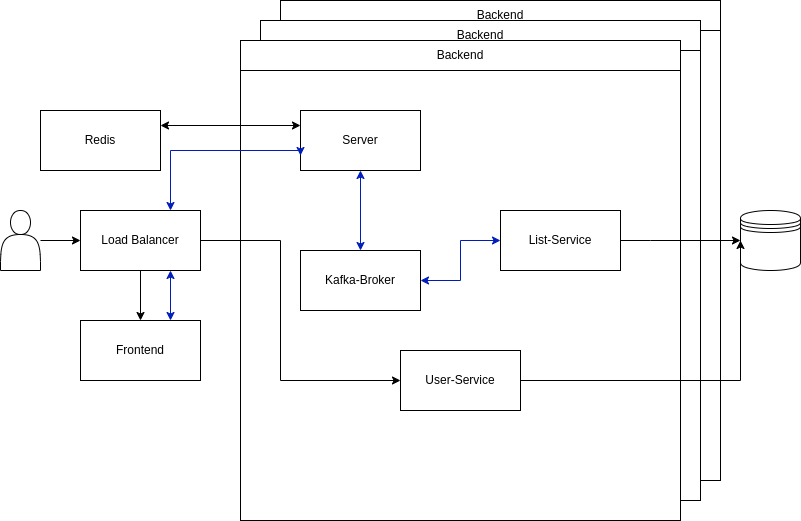
\includegraphics[width=1\linewidth]{resources/images/DistributedSystemDiagram.drawio}
	\caption{Architekturdiagramm der TODO-Listen Anwendung}
	\label{fig:DistributedSystemDiagram.drawio}
\end{figure}

In dem Diagramm ist die grundlegende Architektur der Anwendung zu sehen. Es gibt einen Load-Balancer um die Anfragen die aus dem Frontend kommen auf die Server Komponente zu verteilen und um die Anfragen an die richtige Komponente zu leiten. Aus dem Frontend können Benutzer angelegt werden, dafür wird eine HTTP-Anfrage an die User-Service Komponente über den Load-Balancer gesendet, diese Komponente führt die Transaktion mit der Datenbank aus. Aus dem Frontend wird eine WebSocket-Verbindung mit der Server Komponente aufgebaut, diese wird ebenfalls über den Load-Balancer geleitet. Die Verbindung zu der Server Komponente erfolgt nur mit gültigem JSON Web Token, dieser kann über den Server bezogen werden. Wenn eine Verbindung hergestellt wurde können neue TODO-Listen angelegt werden, dies erfolgt durch das Senden einer Nachricht über den WebSocket. Die Nachricht geht bei dem Server ein und wird dann an das Kafka Cluster gesendet, von dort wird sie von der List-Service Komponente ausgelesen. Wenn die Nachricht valide ist wird die in ihr beschriebene Aktion ausgeführt, eine Aktion ist zum Beispiel das Erstellen einer neuen Liste. Der List-Service sendet nach der Bearbeitung eine Antwort an das Cluster, von dort wird sie von dem Server gelesen und über den WebSocket an das Frontend gesendet. Um die Verbindung mit dem WebSocket über Server Ausfälle hinweg beizubehalten wird eine Session erstellt, die Daten dazu werden in einem Redis-Cache gespeichert. Als Datenbank wurde eine MariaDB verwendet, da die TODO-Listen sich gut mit einem relationalem Schema darstellen lassen. Die Komponenten die in dem Backend Block sind werden für die Skalierung und Ausfallsicherheit repliziert.


\chapter{Kafka}
Um Nachrichten zwischen verschiedenen Komponenten in Echtzeit auszutauschen wird in größeren Systemen Kafka verwendet. Kafka ist eine Event Streaming Plattform die von der Apache Software Foundation bereitgestellt wird. Sie ist eine Open-Source Software. Eingesetzt wird Kafka in Bereichen in denen eine Komponente Daten auswirft und eine andere Komponente diese Daten sofort verarbeiten soll, dieses Szenario tritt in Banksystemen auf wo eine Geldtransaktion so schnell wie möglich verarbeitet werden soll. Wichtig hierbei ist auch die Sicherheit, selbstverständlich sollten keine Transaktionen verloren gehen. Um dies zu vermeiden ist Kafka in der Lage die gesendeten Daten für eine unbegrenzte Zeit zuverlässig zu speichern. Ein anderer Einsatzort von Kafka ist im Internet of Things Bereich, hier werden Sensordaten von den verschiedenen IoT Geräten an Kafka übertragen und von dort kann dann eine Komponente diese Daten auslesen und verarbeiten. Die Skalierbarkeit von Kafka ist ein großer Vorteil. Es können viele produzierende und verarbeitende Komponenten mit Kafka verwendet werden, im IoT Bereich werden viele Geräte Daten senden und diese können dann von wenigen Komponenten verarbeitet werden. Um mit beiden Seiten mit zu skalieren werden sogenannte Cluster in Kafka gebildet. Ein Cluster besteht aus einem oder mehr Kafka Instanzen diese arbeiten zusammen um die Daten zu empfangen, speichern und zu versenden. Für eine erhöhte Ausfallsicherheit und um die Last zu verteilen werden normalerweise immer mindestens drei Kafka Instanzen zusammen verwendet. Dieses Cluster kann falls eine Kafka Instanz ausfällt dies ausgleichen und die Arbeit auf die laufenden Kafka Instanzen verteilen, hierbei gehen auch keine Daten verloren. Die Daten in den Kafka Instanzen, die auch Broker genannt werden, werden repliziert, dass bedeutet mehrere Broker besitzen die gleichen Daten. Dadurch gehen keine Daten verloren selbst wenn ein oder mehr Broker ausfallen. Wenn etwas in dem System passiert, dazu zählen Sensordaten Ermittlung und anstoßen einer Transaktion, wird dies als Event in Kafka festgehalten. Diese Events können auch Nachricht genannt werden, da diese auch zur Übertragung dienen. Ein Producer in Kafka ist eine Anwendung die Events/Nachrichten in das Kafka Cluster schreibt. Die andere Seite wird Consumer genannt, diese Anwendungen lesen die Daten aus dem Kafka Cluster und verarbeiten sie. Durch diese Trennung der Einheiten ist Kafka viel skalierbarer, alle drei Einheiten können unabhängig voneinander skaliert werden. Für gewöhnlich wird das Cluster in der Skalierung an die Consumer und Producer angepasst, da über dieses alle Events durchgehen und es somit mit beiden Seiten mithalten muss. Wenn ein Event in das Cluster eingeht wird es in einem Topic gespeichert, ein Topic ist von der Arbeitsweise ähnlich zu einem normalen Dateiverzeichnis. Alle Topics in Kafka können null, ein oder viele Producer haben und auch null, ein oder viele Consumer haben. Ein unterschied den Topics zu anderen Nachrichtensystemen haben ist das die Events die gespeichert sind nicht nach dem lesen entfernt werden. Ein Event kann so oft wie nötig gelesen werden, dieses Verhalten kann für jedes Topic eingestellt werden. Ebenfalls lässt sich einstellen wie lange die Events gespeichert bleiben sollen bevor sie gelöscht werden. \autocite{ApacheKafka}

\begin{figure}[H]
	\centering
	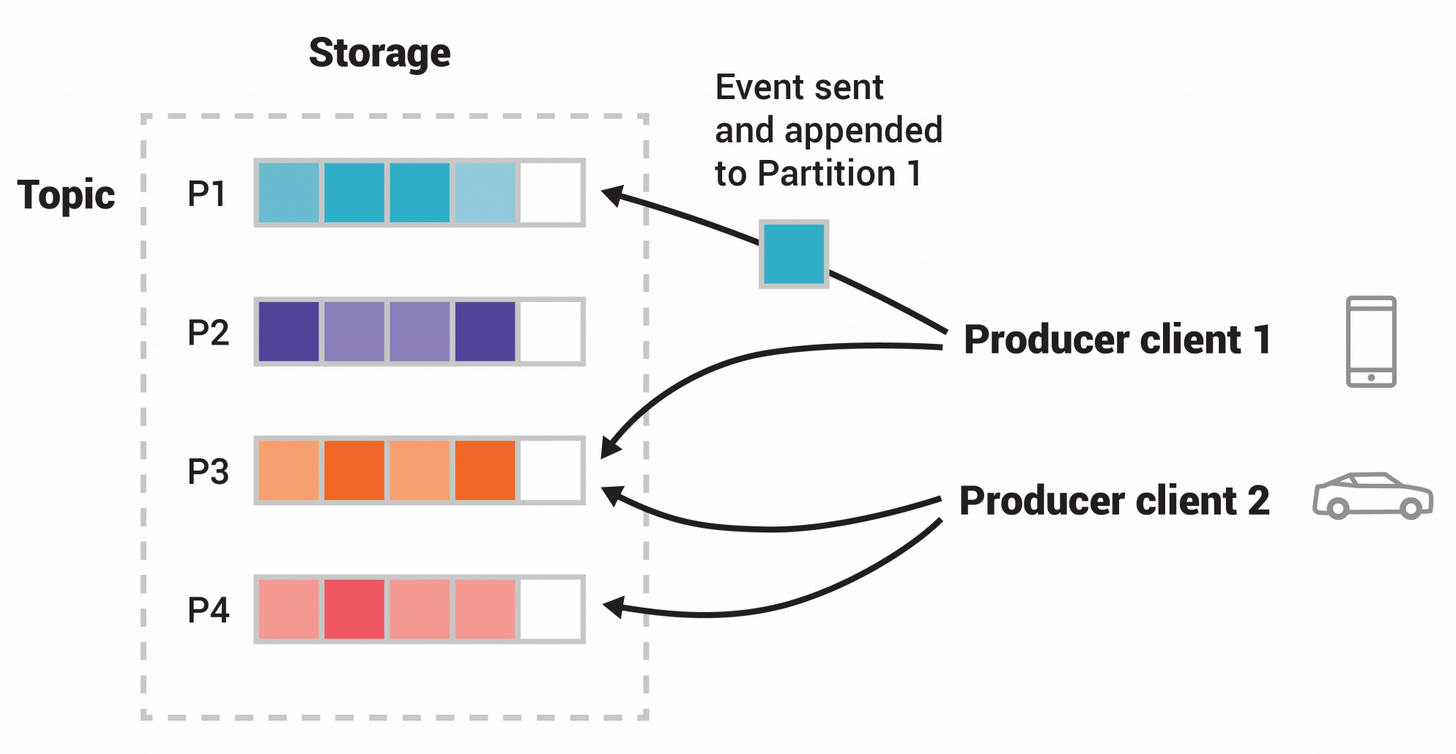
\includegraphics[width=1\linewidth]{resources/images/partition}
	\caption{Hier ist die Partitionierung mit zwei Producern dargestellt.}
	\label{fig:Partition}
\end{figure}

Die Topics sind partitioniert, das bedeutet das Teile des Topics auf verschiedenen Kafka Brokern liegt. Diese Verteilung verbessert die Skalierbarkeit, da in mehreren Brokern gleichzeitig gelesen und geschrieben werden kann. Wie bereits angesprochen können Daten repliziert werden, genauer werden die Topics auf verschiedene Broker repliziert.

In bestimmten Fällen, wie bei Geldtransaktionen, ist es entscheidend, dass Events nur einmal verarbeitet werden, damit keine doppelten Abbuchungen erfolgen. Kafka bietet hierfür Funktionen, die genau einmalige Verarbeitung ermöglichen (exactly-once). Diese Garantie gilt allerdings nur innerhalb des Kafka Systems, also vom Schreiben bis zum Lesen eines Events. Ein wichtiger Mechanismus dabei ist die Idempotenz bei dem Producer. Jeder Producer erhält eine eindeutige ID, und Nachrichten werden mit einer Sequenznummer versehen. Falls es beim Senden zu Fehlern kommt und die Nachricht erneut gesendet wird nimmt Kafka sie nur an, wenn die Sequenznummer direkt auf die vorherige folgt. So wird verhindert, dass Nachrichten mehrfach geschrieben werden. Die Idempotenz gilt jedoch nur für eine Producer Session. Wenn der Producer ausfällt und neu startet, erhält er entweder eine neue ID oder eine neue Epoche, was zu Duplikaten führen kann.

Um sicherzustellen, dass jede Nachricht in jeder Stufe genau einmal verarbeitet wird, kommt die Transaktionsfunktion von Kafka zum Einsatz. Mit ihr können Events atomar in mehrere Topics und Partitionen geschrieben und gleichzeitig die Offsets der konsumierten Nachrichten gespeichert werden. Jede Verarbeitungsstufe liest Events aus einem oder mehreren Quell Topics, führt Berechnungen durch und schreibt die Ergebnisse in Ziel Topics. Mit Kafka Transaktionen lassen sich diese Schritte als eine atomare Einheit zusammenfassen. Obwohl Transaktionen in verteilten Systemen oft komplex sind funktionieren sie in Kafka, da sie sich auf das geschlossene System von Kafka Topics und Partitionen beschränken. Zuletzt müssen die Events aus Kafka heraus in ein anderes System übertragen werden. Um sicherzustellen, dass dies genau einmal passiert wird ein transaktionaler Consumer verwendet. Dabei wird das Ergebnis der Verarbeitung einer Nachricht zusammen mit dem Offset als atomare Einheit im Zielsystem gespeichert. \autocite{ExactlyOnce}

\section{Einsatz}
In der TODO-Listen Anwendung wird Kafka benutzt um Nachrichten von der Server Komponente zu der List-Service Komponente zu übertragen und die Antwort ebenfalls wieder zu übertragen. Da sowohl Server als auch List-Service repliziert werden war es wichtig Events genau einmal zu verarbeiten, da der List-Service anhand der Events die er erhält Aktionen in der Datenbank ausführt. Wenn der Benutzer im Frontend eine neue Liste hinzufügen möchte könnte ohne die exactly-once Semantik die Liste mehrfach erstellt werden. Die Nachricht wird aus dem Kafka Cluster von allen Repliken des List-Service gelesen und alle führen die Aktion auf der Datenbank aus. Dies ist natürlich nicht korrekt. Der Benutzer wird sicherlich nicht zufrieden sein wenn er eine Liste anlegen will und am Ende drei oder mehr mit den gleichen Angaben hat. Damit diese mehrfach Erstellung der Listen und Elemente nicht eintritt wird sichergestellt das jedes Event genau einmal verarbeitet wird. Wichtig dabei war zu beachten das der Replikationsfaktor für Kafka erhöht werden muss, dass bedeutet in dem Cluster müssen mindestens drei Broker sein. Durch die Replikation der Broker und den Topics wird sichergestellt das Events und somit auch Datenbankaktionen genau einmal verarbeitet werden. Die Implementierung von Kafka in das System war durch das Spring Boot Framework nicht sehr kompliziert, jedoch benötigt Kafka ein gewisses Verständnis und bestimmte Codeteile sind oft sehr ähnlich. Kafka ist äußerst performant und zuverlässig, die Nachrichten werden in wenigen Millisekunden übertragen und keine Nachricht ist verloren gegangen. Die Aufteilung in Producer, Broker/Cluster und Consumer macht Kafka nicht nur sehr skalierbar, sondern hilft auch dem Verständnis. Da alle Interessenbereiche separat gehalten werden und genau klar ist was für welche Funktion zuständig ist. Nachdem die Grundlagen gut verstanden wurden ist die Spezifizierung an das eigene System gut möglich und Kafka bietet eine riesige Anzahl an Konfigurationsmöglichkeiten, beinahe jede Kleinigkeit lässt sich individuell konfigurieren.

\chapter{WebSocket}
WebSocket ist ein W3C-Standard (RFC 6455) aus dem Jahr 2011, der eine bidirektionale und vollduplexe Kommunikation zwischen Client und Server ermöglicht. Im Gegensatz zur traditionellen HTTP Kommunikation, erlaubt WebSocket eine aktive Kommunikation beider Seiten über eine einzelne, persistente TCP-Verbindung. Dies wird mit einem spezielles Protokollhandshake gemacht, bei dem eine bestehende HTTP-Verbindung auf WebSocket upgegraded wird. Nach diesem Upgrade können Daten effizienter ausgetauscht werden, ohne erneute HTTP-Anfragen. \autocite{WebSocketW3C} \autocite{WebSocketHeise}

\section{Funktionsweise}
Die WebSocket-Kommunikation beginnt mit einer GET-Anfrage des Clients, in der wird das Upgrade auf das WebSocket-Protokoll explizit gefordert. Der Server akzeptiert diesen Wechsel, signalisiert dies durch den HTTP-Statuscode 101 und öffnet die Verbindung. Ab jetzt verwenden beide Seiten einen bidirektionalen Kommunikationskanal, der durch das WebSocket-Protokoll geregelt wird. Dabei können Nachrichten in Echtzeit ausgetauscht werden, ohne den Overhead traditioneller HTTP-Anfragen. WebSocket verwendet standardmäßig die Ports 80 und 443. \autocite{WebSocketW3C}

\section{Handshake-Prozess}
Der Handshake-Prozess zwischen Client und Server läuft in diesen Schritten ab. In der initialen Anfrage sendet der Client eine GET-Anfrage, in der signalisiert er den Wechsel zum WebSocket-Protokoll. Dies geschieht durch Header wie Upgrade und Connection: Upgrade. Bei der Schlüssel-Validierung generiert der Client einen Base64-codierten Schlüssel, der als Sec-WebSocket-Key an den Server gesendet wird. Der Server nutzt diesen Schlüssel, um eine Antwort zu generieren, die er an den Client zurückgibt. Wenn der Server antwortet signalisiert er den Wechsel des Protokolls durch die Rückgabe des HTTP-Statuscodes 101 (Switching Protocols) sowie durch das Hinzufügen des berechneten Schlüssels (Sec-WebSocket-Accept) in den Headern seiner Antwort.Sobald der Client die Antwort des Servers erhält wird die Verbindung auf das WebSocket-Protokoll umgestellt, nun ist ein bidirektionaler Datentransfer möglich. \autocite{WebSocketHeise}

\section{Einsatz im Backend}
Eine WebSocket-Verbindung wird mit dem Frontend aufgebaut und über diese werden Nachrichten ausgetauscht. Die Nachrichten benötigen ein bestimmtes Format, damit diese direkt über Kafka weitergesendet werden können. Der WebSocket kann als eine simplere Erweiterung von Kafka im Backend gesehen werden. Nachrichten die im Server eingehen werden mit einer zufällig generierten UUID ausgestattet und dann über Kafka versendet. Die Antwort des List-Service geht im Server ein und wird eins zu eins über den WebSocket weitergeleitet. Ein WebSocket wurde eingesetzt um die Übertragung in Echtzeit zu haben, da Listen Änderungen sofort aktualisiert werden sollen. Durch die bidirektionale Kommunikation können Nachrichten in beide Richtungen übertragen werden ohne das diese sich gegenseitig blockieren, somit ist die TODO-Liste reaktiver auf die Änderungen die von dem Benutzer ausgehen. Im Backend war die Implementierung der WebSocket-Unterstützung recht einfach. Der WebSocket arbeitet wie Kafka mit Topics, aber bei dem WebSocket sind diese Topics eher als Ziele zu verstehen. Ein WebSocket kann ein bestimmtes Topic subscriben und erhält automatisch alle Nachrichten die an dieses Topic gerichtet sind, allerdings werden die Nachrichten nirgendwo gespeichert und sind nach dem lesen weg. Das Senden und Empfangen von Nachrichten erweist sich mit den Spring Boot Framework als sehr einfach, da es schon reicht die richtigen Annotations mit den richtigen Routen über eine Funktion zu setzen. Beim Empfangen wird die Funktion mit der Annotation aufgerufen und ihr wird der Inhalt der Nachricht im Parameter übergeben, hier kann bereits eine bestimmte Nachrichtenform definiert werden. Die Funktion kann dann die Nachrichten verarbeiten, im Fall der TODO-Listen Anwendung wird die Nachricht mit einer UUID erweitert und anschließend an das Kafka Cluster gesendet. Beim Empfangen von Nachrichten von Kafka wird eine andere Funktion ausgeführt, bei dieser wird einfach die Kafka Nachricht direkt an den Client gesendet. Die WebSocket-Verbindung mit einem JWT zu versehen war ziemlich einfach, das meiste wird durch Konfigurationsdateien gemacht. Es sind sicherlich noch viele Erweiterungen mit WebSockets und Kafka machbar und die beiden bieten eine große Anwendungsfläche.

    %% Literaturverzeichnis
    \printbibliography[title=Literaturverzeichnis]
    \clearpage


\end{document}
